% Copyright 2012 David W. Hogg (NYU).  All rights reserved.

\documentclass[pdftex]{beamer}
\usepackage{amssymb,amsmath,mathrsfs}
\usecolortheme{default}

% this one is debatable
\renewcommand{\emph}[1]{\textbf{#1}}

%%% color commands
\newcommand{\whiteonblack}{%
  \colorlet{fg}{white}
  \colorlet{bg}{black}
  \setbeamercolor{normal_text}{fg=white,bg=black}
  \setbeamercolor{background canvas}{fg=white,bg=black}
  \setbeamercolor{alerted_text}{fg=yellow}
  \setbeamercolor{example_text}{fg=white}
  \setbeamercolor{structure}{fg=white}
  \setbeamercolor{palette_quaternary}{fg=white}
}
\newcommand{\blackonwhite}{%
  \colorlet{fg}{black}
  \colorlet{bg}{white}
  \setbeamercolor{normal_text}{fg=black,bg=white}
  \setbeamercolor{background canvas}{fg=black,bg=white}
  \setbeamercolor{alerted_text}{fg=blue}
  \setbeamercolor{example_text}{fg=black}
  \setbeamercolor{structure}{fg=black}
  \setbeamercolor{palette_quaternary}{fg=black}
}
\xdefinecolor{pink}{rgb}{1.0,0.9,0.9}

%%% size and shape commands
\newlength{\figurewidth}
\setlength{\figurewidth}{0.9\textwidth}
\newlength{\figureheight}
\setlength{\figureheight}{0.9\textheight}

%%% text commands
\newcommand{\project}[1]{\textsl{#1}}
  \newcommand{\an}{\project{Astrometry.net}}
  \newcommand{\tc}{\project{The~Cannon}}
  \newcommand{\euclid}{\project{Euclid}}
  \newcommand{\flickr}{\project{flickr}}
  \newcommand{\gaia}{\project{Gaia}}
  \newcommand{\galex}{\project{GALEX}}
  \newcommand{\kepler}{\project{Kepler}}
  \newcommand{\GALEX}{\galex}
  \newcommand{\hst}{\project{HST}}
  \newcommand{\hipparcos}{\project{Hipparcos}}
  \newcommand{\lsst}{\project{LSST}}
  \newcommand{\sdss}{\project{SDSS}}
  \newcommand{\sdssiii}{\project{SDSS-III}}
  \newcommand{\sdssiv}{\project{SDSS-IV}}
  \newcommand{\boss}{\sdssiii\ \project{BOSS}}
  \newcommand{\osss}{\project{OSSS}}
  \newcommand{\ska}{\project{SKA}}
  \newcommand{\vo}{\project{VO}}
  \newcommand{\rttd}{\project{Right Thing To Do}$^{\mbox{\scriptsize\sffamily{TM}}}$}
\newcommand{\foreign}[1]{\textit{#1}}
\newcommand{\latin}[1]{\foreign{#1}}
  \newcommand{\cf}{\latin{cf.}}
  \newcommand{\eg}{\latin{e.g.}}
  \newcommand{\etal}{\latin{et~al.}}
  \newcommand{\etc}{\latin{etc.}}
  \newcommand{\ie}{\latin{i.e.}}
  \newcommand{\vs}{\latin{vs.}}

%%% math-mode commands
\newcommand{\unit}[1]{\mathrm{#1}}
  \newcommand{\rad}{\unit{rad}}
  \newcommand{\s}{\unit{s}}
  \newcommand{\yr}{\unit{yr}}
  \newcommand{\km}{\unit{km}}
  \newcommand{\kmps}{\km\,\s^{-1}}
\newcommand{\mmatrix}[1]{\boldsymbol{#1}}
\newcommand{\tv}[1]{\boldsymbol{#1}}
\newcommand{\dd}{\mathrm{d}}
\newcommand{\given}{\,|\,}
\newcommand{\Teff}{T_{\mathrm{eff}}}
\newcommand{\logg}{\log g}
\newcommand{\vsini}{v\,\sin i}
 % hogg standard colors
\setlength{\paperheight}{3.5in}
% 1.77778 is the ratio of 16 to 9
\setlength{\paperwidth}{1.77778\paperheight}
\setlength{\textwidth}{0.85\paperwidth}
\usepackage{amssymb,amsmath,mathrsfs}

\title{1.~hierarchical probabilistic inference \\ {\small and} \\ 2.~the costs and benefits of sharing data}
\author[David W. Hogg (NYU)]{David W. Hogg \\
  \textsl{\small Center for Cosmology and Particle Physics,
                 New York University}}
\date{2012 November 29}

\begin{document}

\begin{frame}
  \titlepage
\end{frame}

\begin{frame}
  \frametitle{infer dynamics from kinematics {\small (0903.5308)}}
  \begin{itemize}
  \item \project{Gaia} will give a snapshot of positions and
    velocities for $10^7$ to $10^9$ stars.  How do we figure out the
    gravitational potential of the Galaxy?
  \item<2-> Let's start by doing this in the Solar System.
  \item<2-> If we can't do the \emph{Solar System} we can't do anything!
  \item<2-> Imagine that you had a \emph{snapshot} of the planet positions
    and velocities on 2009~April~1.
  \item<2-> Could you infer that the force law is $1/r^2$~?
  \end{itemize}
\end{frame}

\begin{frame}
  \frametitle{infer dynamics from kinematics {\small (0903.5308)}}
  \begin{itemize}
  \item In steady-state, $f(\tv{x},\tv{v})$ is a function of conserved
    quantities only.
  \item $\displaystyle
        p(\tv{x}_i,\tv{v}_i|\tv{\omega},\tv{\alpha})
      = \left|\left|\frac{\dd\tv{I}\,\dd\tv{\phi}}{\dd\tv{x}\,\dd\tv{v}}\right|\right|_{\tv{\omega}}\,\left[\frac{1}{2\pi}\right]^3
      \,p(\tv{I}|\tv{\alpha})$
  \item<2-> $\displaystyle
        p(\tv{x}_i,\tv{v}_i|\tv{\omega})
      = \int \dd\tv{\alpha}\,p(\tv{\alpha})
      \,p(\tv{x}_i,\tv{v}_i|\tv{\omega},\tv{\alpha})$
  \item<2-> Marginalization is hard:
    \begin{itemize}
    \item 200 parameters in the marginalization
    \item more parameters than data!
    \item priors from Gaussian processes
    \end{itemize}
  \end{itemize}
\end{frame}

\begin{frame}
  \frametitle{infer dynamics from kinematics {\small (0903.5308)}}
  \includegraphics[width=\textheight]{../../pgm/gaia.pdf}
\end{frame}

\newlength{\jacwidth}
\setlength{\jacwidth}{0.25\textwidth}

\begin{frame}
  \frametitle{infer dynamics from kinematics {\small (0903.5308)}}
  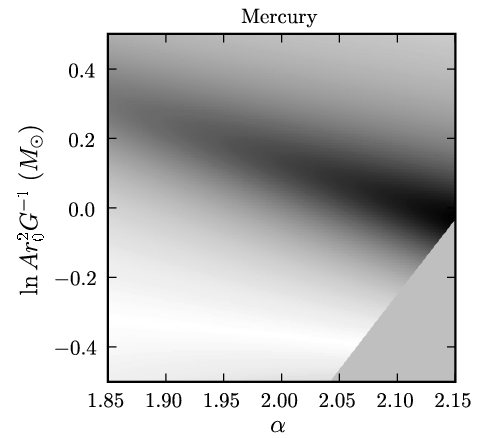
\includegraphics[width=\jacwidth]{jacobian-3.png}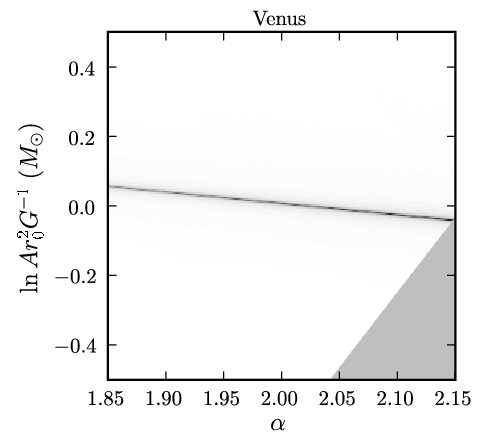
\includegraphics[width=\jacwidth]{jacobian-7.png}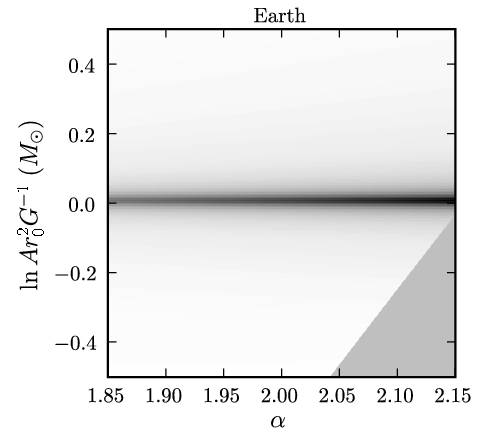
\includegraphics[width=\jacwidth]{jacobian-0.png}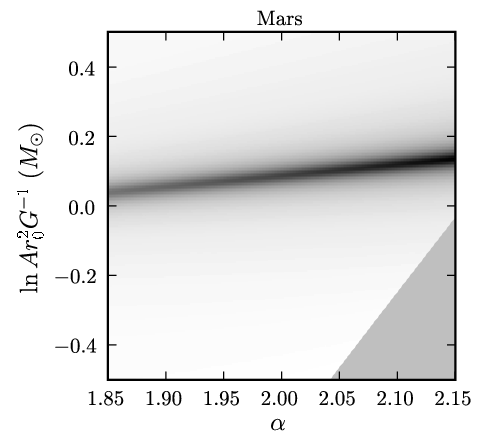
\includegraphics[width=\jacwidth]{jacobian-2.png} \\
  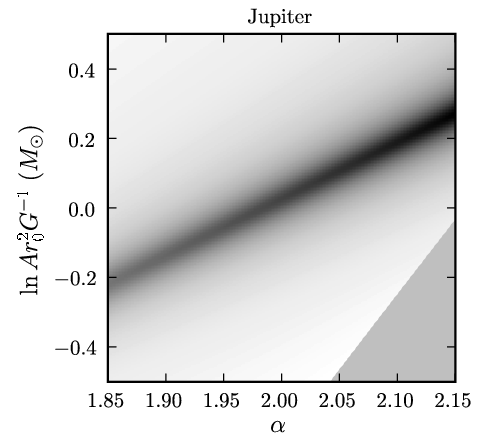
\includegraphics[width=\jacwidth]{jacobian-1.png}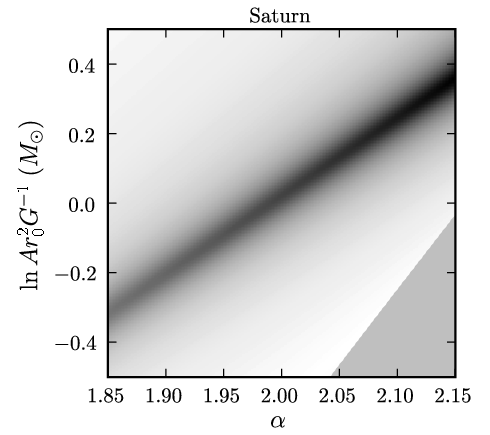
\includegraphics[width=\jacwidth]{jacobian-5.png}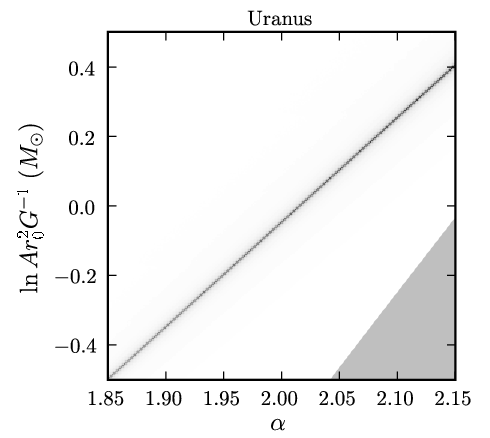
\includegraphics[width=\jacwidth]{jacobian-6.png}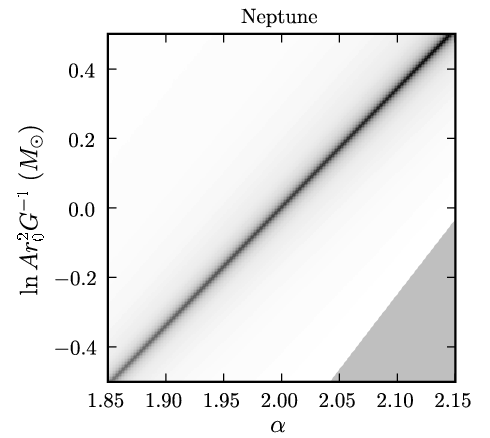
\includegraphics[width=\jacwidth]{jacobian-4.png}
\end{frame}

\begin{frame}
  \frametitle{infer dynamics from kinematics {\small (0903.5308)}}
  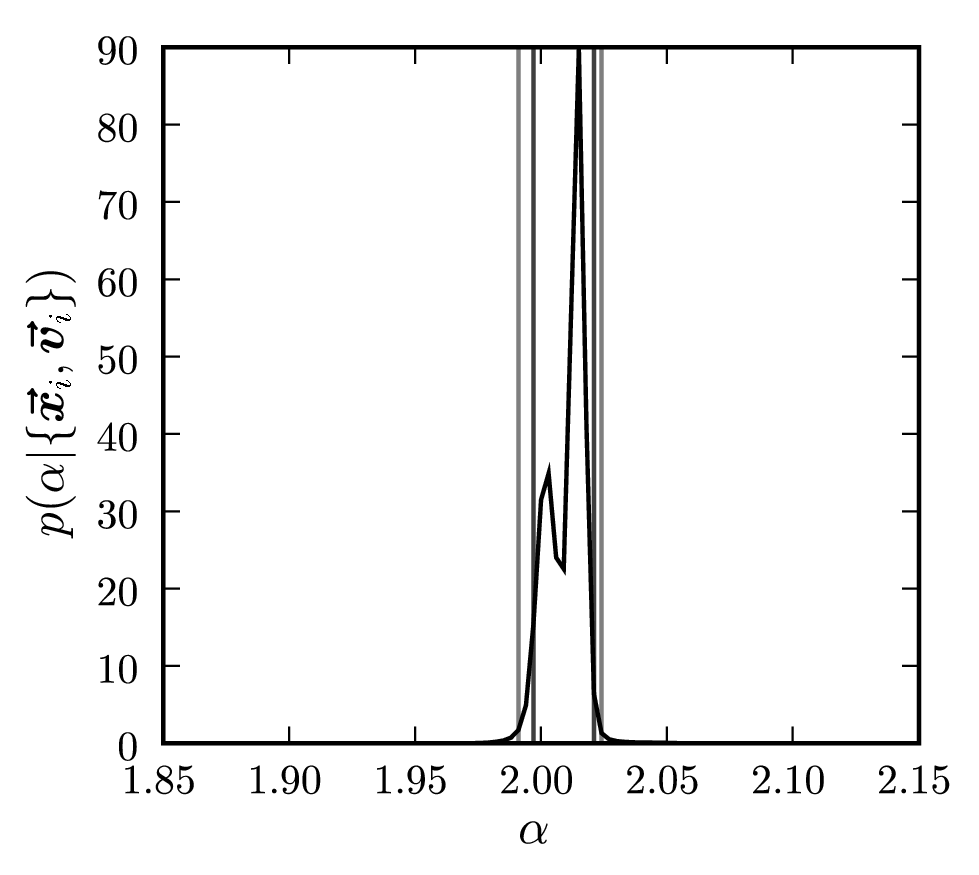
\includegraphics[width=\textheight]{alpha.png}
\end{frame}

\begin{frame}
  \frametitle{infer dynamics from kinematics {\small (0903.5308)}}
  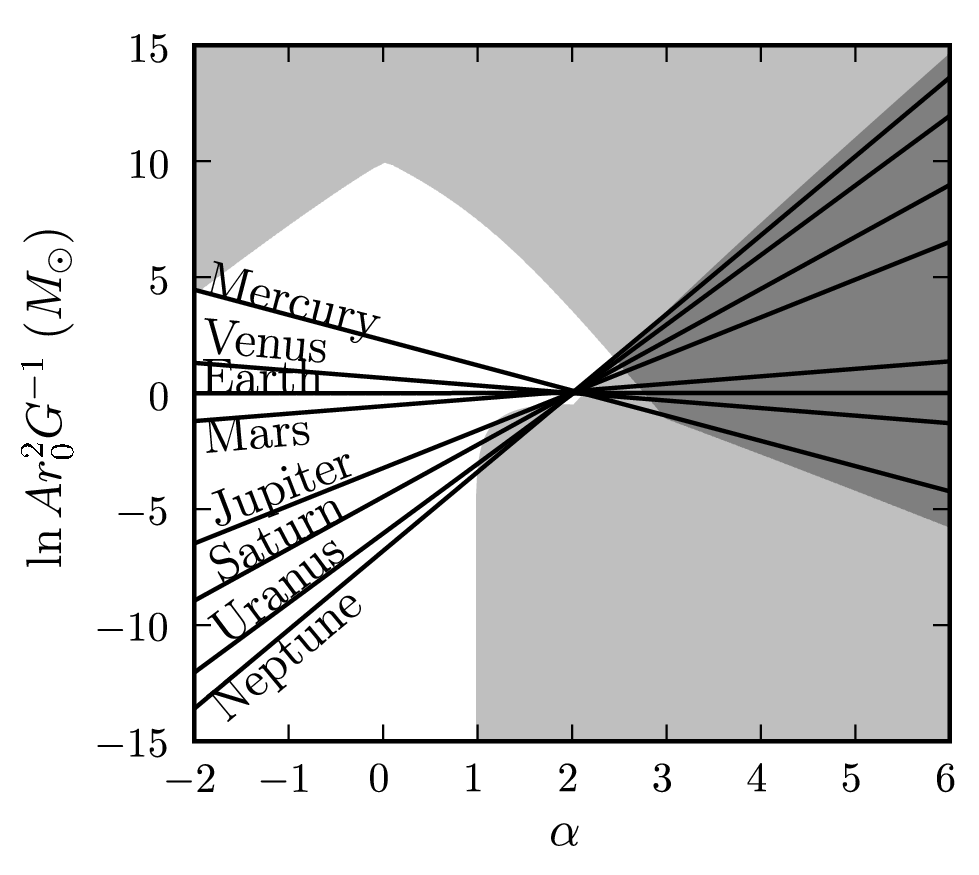
\includegraphics[width=\textheight]{virial.png}
\end{frame}

\begin{frame}
  \frametitle{infer dynamics from kinematics {\small (0903.5308)}}
  \begin{itemize}
  \item The phase-space DF model is so general, it can \emph{discover}
    phase-space structure.
  \item There \emph{is} phase-space structure.
  \item All currently used point estimates---even maximum-likelihood
    ones---either have this hard-coded (bad) or can't discover it
    (bad).
  \item (That said, the procedure was \emph{expensive}.)
  \end{itemize}
\end{frame}

\begin{frame}
  \frametitle{models of no fixed complexity {\small (1211.5805)}}
  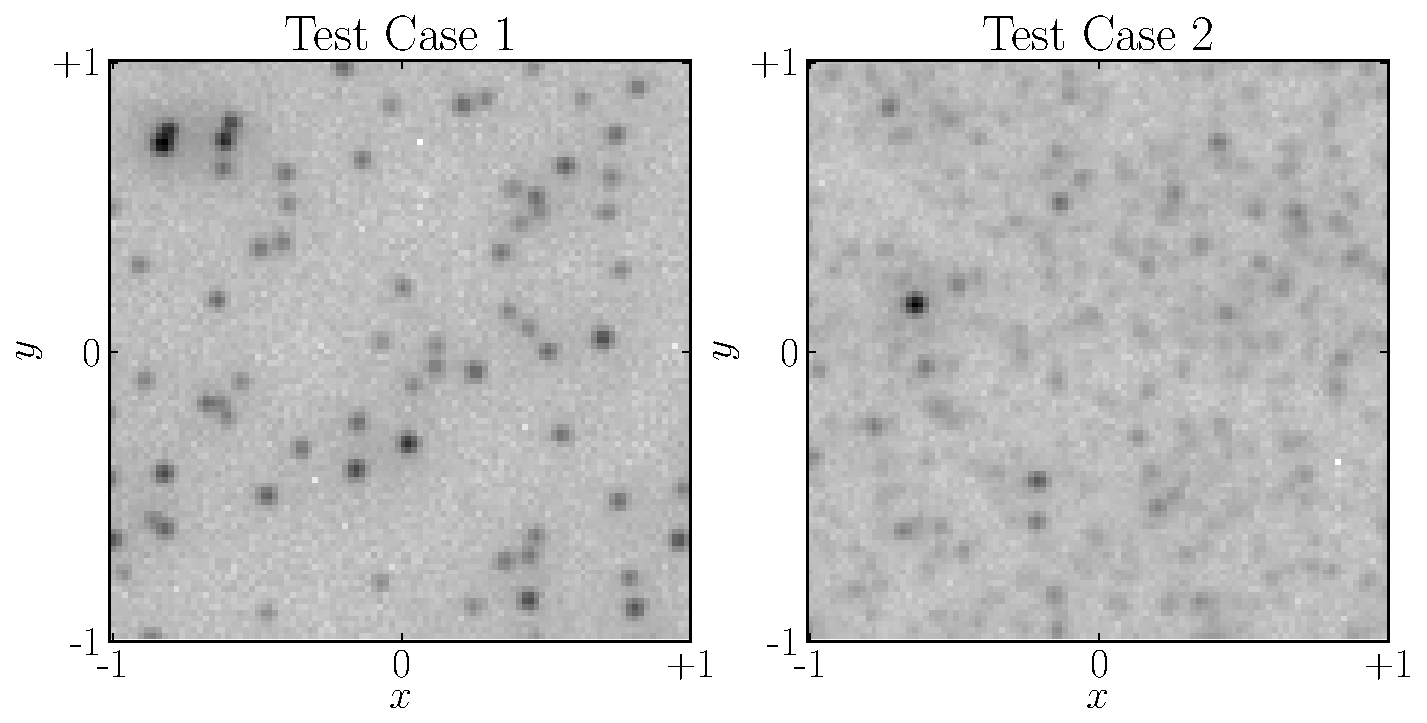
\includegraphics[width=\textwidth]{test_cases_copy.pdf}
\end{frame}

\begin{frame}
  \frametitle{models of no fixed complexity {\small (1211.5805)}}
  \begin{itemize}
  \item Images filled with stars; want to know the luminosity function of stars.
  \item Catalog \emph{itself} is a very large blob of nuisance parameters.
  \item Don't know (and don't care) precisely how many stars there are.
  \item Faint stars contribute to the noise.
  \item connections to LIGO:
    \begin{itemize}
    \item ``faint stars'' could be fainter GW sources
    \item ``faint stars'' could be seismic events
    \end{itemize}
  \end{itemize}
\end{frame}

\begin{frame}
  \frametitle{models of no fixed complexity {\small (1211.5805)}}
  \includegraphics[width=\textheight]{../../pgm/crowded.pdf}
\end{frame}

\begin{frame}
  \frametitle{models of no fixed complexity {\small (1211.5805)}}
  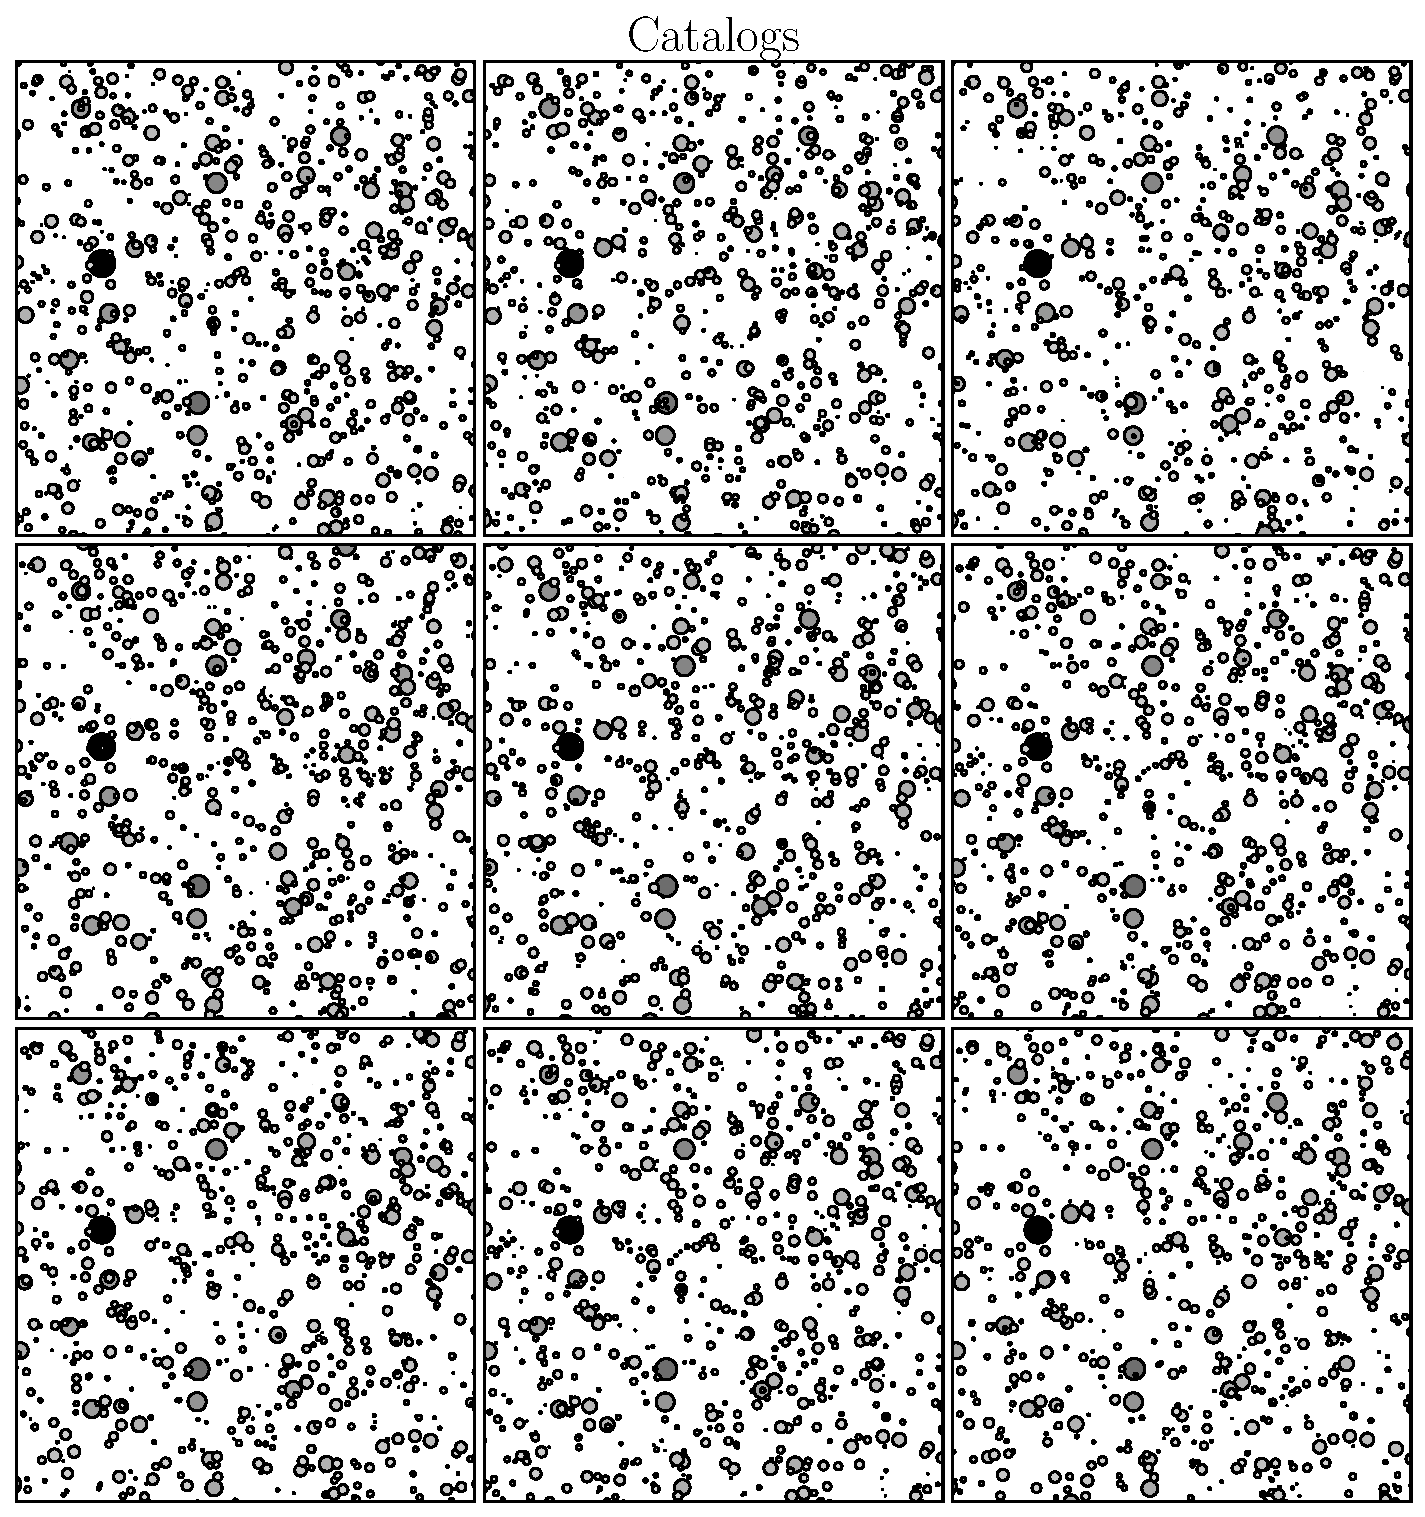
\includegraphics[width=\textwidth]{catalogs_copy.pdf}
\end{frame}

\begin{frame}
  \frametitle{models of no fixed complexity {\small (1211.5805)}}
  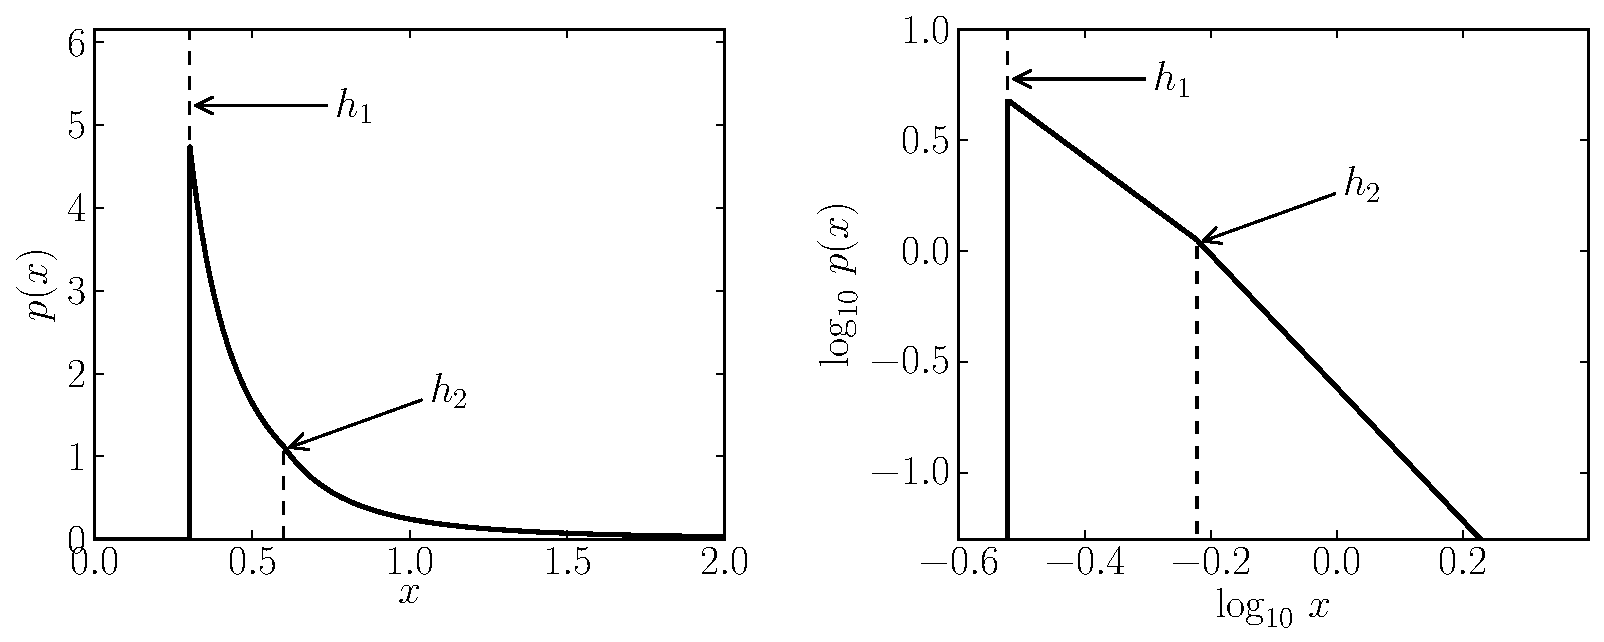
\includegraphics[height=0.45\textheight]{broken_copy.pdf}\\
  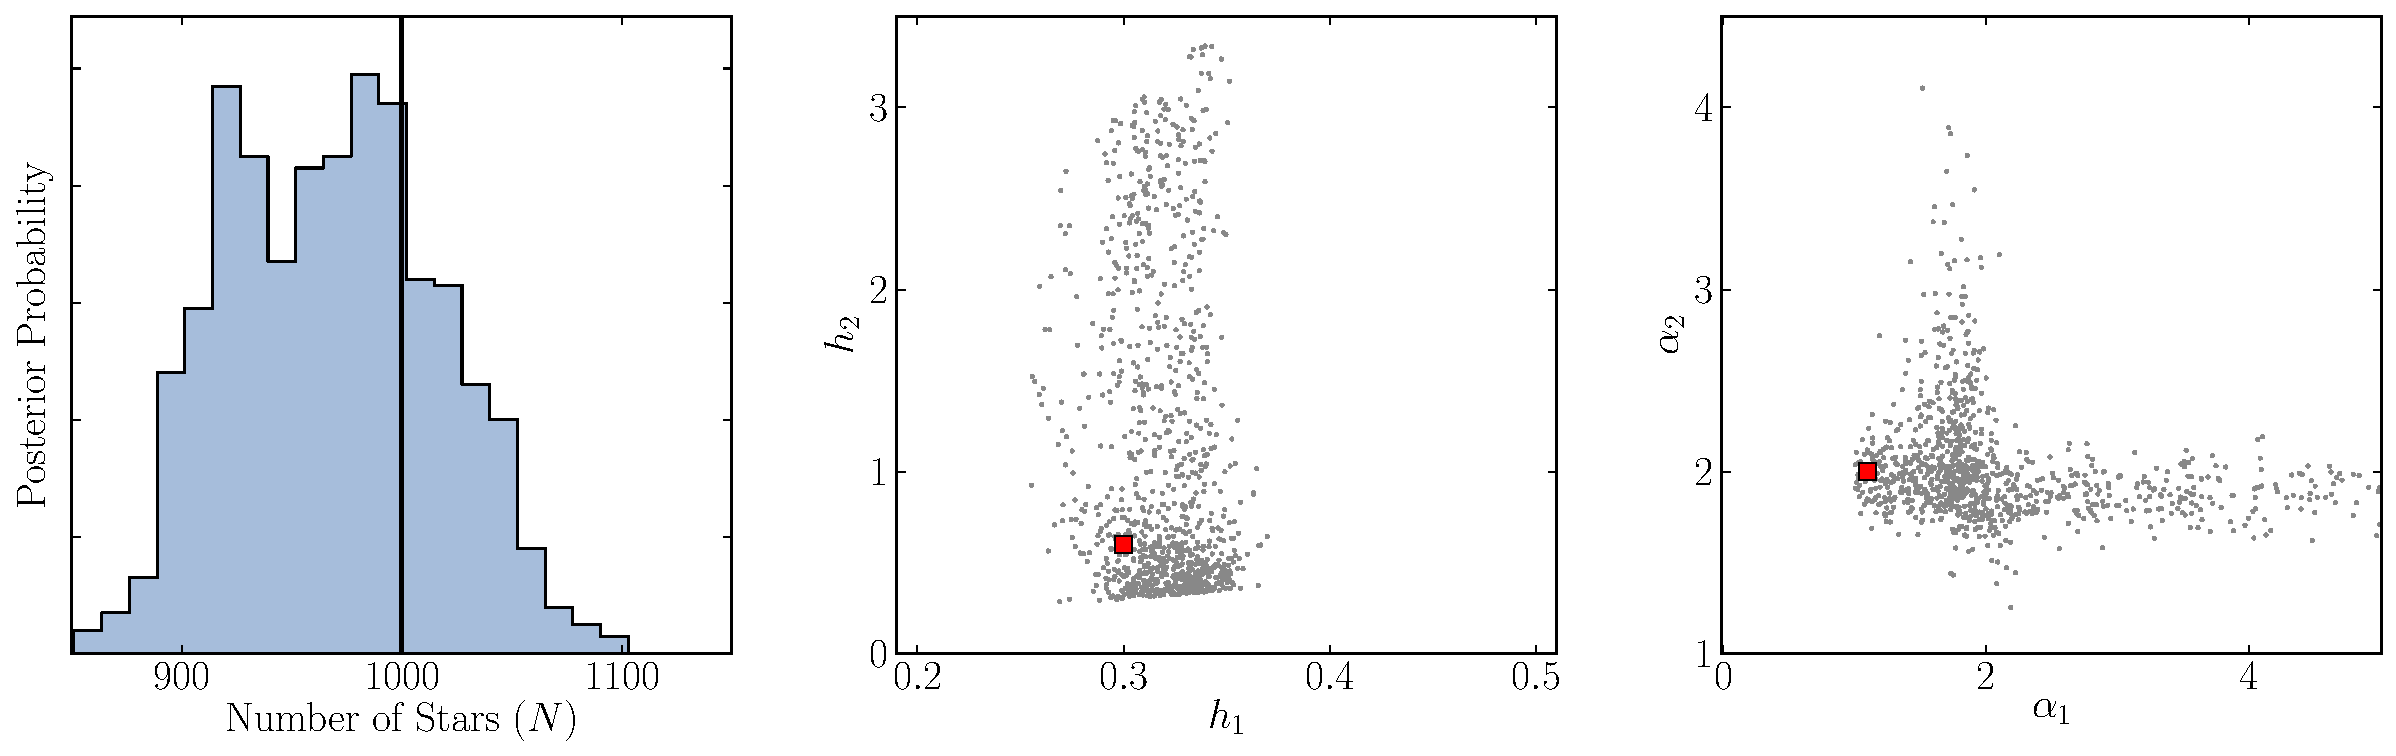
\includegraphics[height=0.45\textheight]{inference2_copy.pdf}
\end{frame}

\begin{frame}
  \frametitle{latent time-domain models {\small Listgarten \etal, NIPS 2004}}
  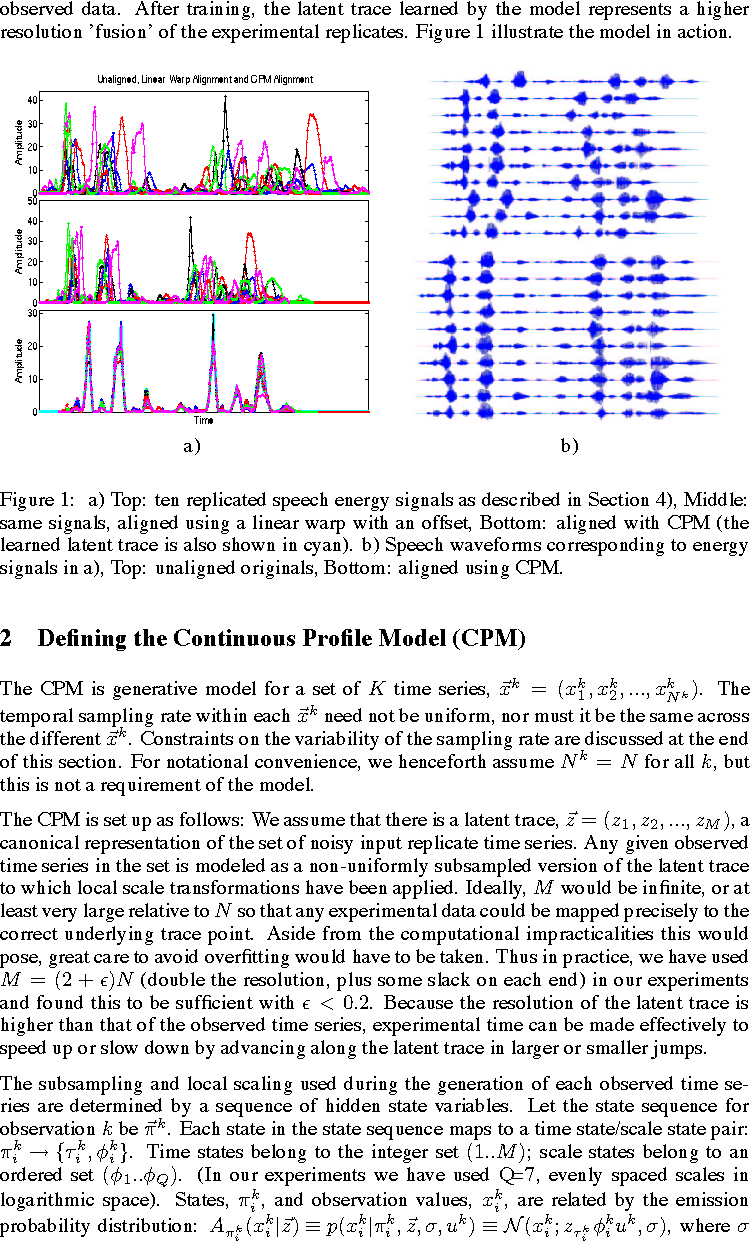
\includegraphics[trim=0 0in 0 0.4in, clip, width=\textwidth]{alignment_nips2004_sound-crop.pdf}
\end{frame}

\begin{frame}
  \frametitle{latent time-domain models {\small Listgarten \etal, NIPS 2004}}
  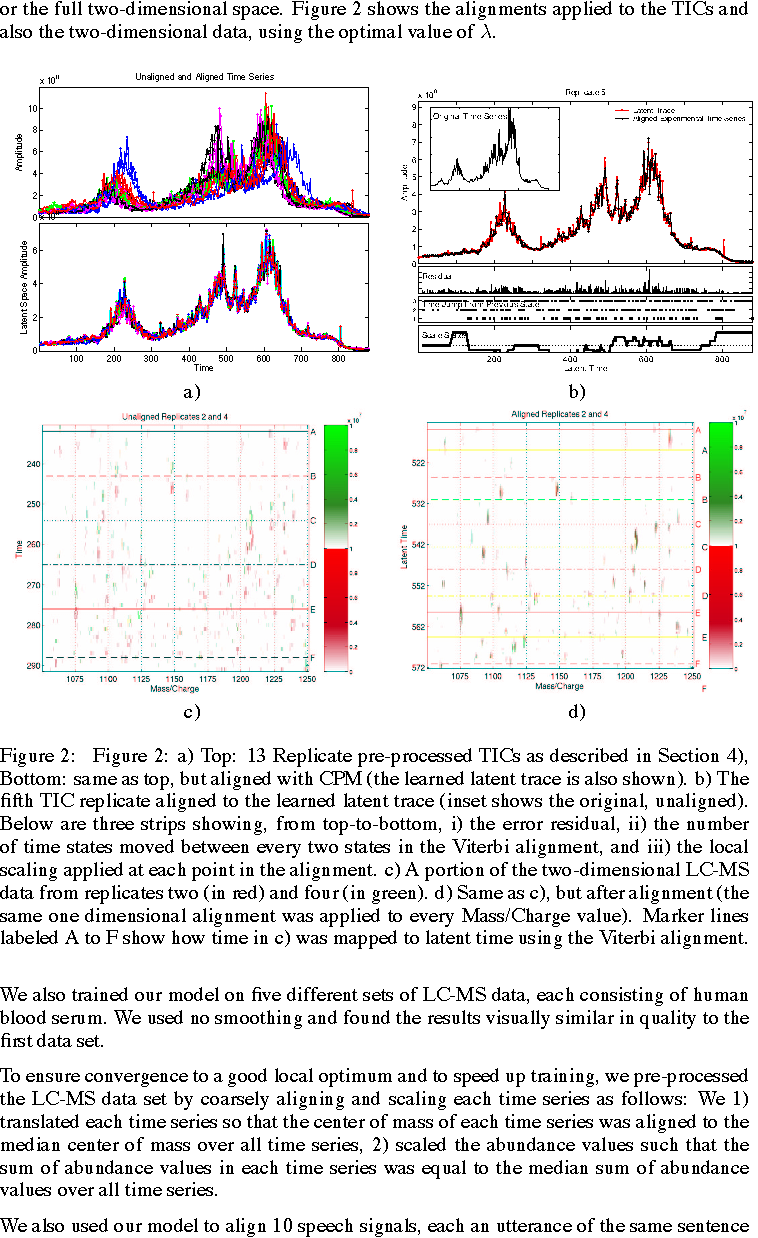
\includegraphics[trim=0 0in 0 0.4in, clip, width=\textwidth]{alignment_nips2004_chrom-crop.pdf}
\end{frame}

\begin{frame}
  \frametitle{latent time-domain models {\small Listgarten \etal, NIPS 2004}}
  \begin{itemize}
  \item There is a latent ``true'' time-domain function.
  \item There is a set of free ``time warping'' functions.
  \item More parameters than data (truly non-parametric).
  \item connections to LIGO:
    \begin{itemize}
    \item small wrongnesses in template can make template orthogonal to signal
    \item very good ideas about priors or regularization
    \end{itemize}
  \end{itemize}
\end{frame}

\begin{frame}
  \frametitle{conclusions 1: hierarchical inference}
  \begin{itemize}
  \item Hierarchical inference makes experiments more accurate and precise.
    \begin{itemize}
    \item ``Data-driven regularization''.
    \item The prior for each data point is informed by all other data points.
    \item Often it is only the \emph{hyperparameters} that you care about.
    \end{itemize}
  \item Expect to spend a huge number of parameters on nuisances.
    \begin{itemize}
    \item Don't be afraid to have more parameters than data.
    \item Don't like priors?  You only need them on your nuisance parameters.
    \end{itemize}
  \end{itemize}
\end{frame}

\begin{frame}
  \frametitle{the costs of sharing data}
  \begin{itemize}
  \item The data are so damned complicated; who outside the collaboration could understand?
  \item Data stewardship and serving is expensive and complexifies the project.
  \item Stupid people will write stupid papers and that will reflect badly on the project.
  \item We will have to spend our time answering helpdesk queries and swatting down dumb papers.
  \item This is an experiment; if you want to repeat it, build your own damned \project{LIGO}.
  \end{itemize}
\end{frame}

\begin{frame}
  \frametitle{Sloan Digital Sky Survey}
  \begin{itemize}
  \item \project{Early Data Release} and \project{DR1} had massive issues.
  \item Found flat-field problem, fixed it
    \begin{itemize}
    \item eventually reached unheard-of photometric precision
    \end{itemize}
  \item Openness within the Collaboration was also invaluable.
    \begin{itemize}
    \item \project{SDSS} had no reserved or allocated science
    \end{itemize}
  \item The Collaboration was not filled with morons.
  \end{itemize}
\end{frame}

\begin{frame}
  \frametitle{Hipparcos}
  \begin{itemize}
  \item Unprecedented high-precision astrometric mission run by the \emph{best people in the world}.
  \item Produced a single data release: One final Catalog.
  \item Issues found with distance scale by outside analyses of the Catalog
  \item Independent re-analysis is now the go-to Catalog.
    \begin{itemize}
    \item the official \project{Hipparcos} Catalog is now \emph{deprecated}.
    \end{itemize}
  \end{itemize}
\end{frame}

\begin{frame}
  \frametitle{Wilkinson Microwave Anisotropy Probe}
  \begin{itemize}
  \item Re-analysis of the anomalous quadrupole in the time-stream data.
    \begin{itemize}
    \item probably wrong
    \end{itemize}
  \item The ``Haze''.
    \begin{itemize}
    \item definitely right
    \end{itemize}
  \item The project spent some time bashing both results, unofficially.
  \end{itemize}
\end{frame}

\begin{frame}
  \frametitle{benefits of sharing data}
  \begin{itemize}
  \item Science is the \emph{ultimate functional testing environment}.
    \begin{itemize}
    \item observatories are too complicated for any closed team to find all issues
    \item openness within and without is the only way to get every possible effect tested
    \item managers rarely believe this---they are paid to disbelieve
    \end{itemize}
  \item Good will.
  \item Impact.
  \end{itemize}
    \begin{itemize}
    \item \project{HST}, \project{Spitzer}, \project{GALEX}, and \project{SDSS} all have more archival papers than Team papers.
    \item data release papers have citation rates in the \emph{thousands}
    \end{itemize}
\end{frame}

\begin{frame}
  \frametitle{what to release}
  \begin{itemize}
  \item There are raw data, meta data, calibrated data, events, likelihood functions, and so on.
  \item You get more benefits if you release rawer data.
  \item You feel more pain if you release rawer data.
    \begin{itemize}
    \item code is the best documentation of data
    \item data release without code release is almost useless to you and the public
    \end{itemize}
  \end{itemize}
\end{frame}

\begin{frame}
  \frametitle{licensing}
  \begin{itemize}
  \item Consider conditional releases:
    \begin{itemize}
    \item registration and escrow requirements
    \item comment rights
    \item (bad) reserved science
    \item (bad) MOUs
    \end{itemize}
  \end{itemize}
\end{frame}

\begin{frame}
  \frametitle{conclusions 2: sharing data}
  \begin{itemize}
  \item The costs of sharing are high.
    \begin{itemize}
    \item specific costs are easy to anticipate
    \end{itemize}
  \item The benefits of sharing are high.
    \begin{itemize}
    \item \emph{specific benefits are impossible to anticipate}
    \end{itemize}
  \item The expected functional testing benefit outweighs cost.
    \begin{itemize}
    \item short-term pain is compensated by long-term \emph{non-wrongness}
    \end{itemize}
  \end{itemize}
\end{frame}

\end{document}
